%%%%%%%%%%%%%%%%%%%%%%%%%%%%%%%%%%%%%%%%%%%%%%%%%%%%%%%%%%%%%%%%%%%
%                                                                 %
%                            CHAPTER                              %
%                                                                 %
%%%%%%%%%%%%%%%%%%%%%%%%%%%%%%%%%%%%%%%%%%%%%%%%%%%%%%%%%%%%%%%%%%%

\chapter{Literature study}
In this chapter we will take a quick look at how convolutional neural networks function, layer by layer. We will also learn how secure multiparty computation (MPC) in general is possible. Finaly, we will show the related work on combining these two subjects so far.

\section{Convolutional neural network}
Convolution neural networks (CNN) is a special type of neural network used for images. The spatial properties of the pixels in the image are used during the evaluation of the input, meaning the neighbouring pixels of a central pixel impact the output to the next layer of that central pixel while pixels further away do not.
CNNs are made of multiple layers. Typically, as you move further from the input layer to the output layer the dimensionality reduces, we can say the input gets mapped on a desired output manifold. Inputs that we classify as similar are supposed to be in the same region in the output manifold.

\subsection{Convolution layer}
In this layer a discrete convolution of a kernel $K$ shifting over an image $I$ is performed, as shown in equation \ref{eq:1}. The kernel has parameters also called weights, so that certain features get extracted from the input.
\begin{equation} \label{eq:1}
  (I*K)[m,n]=\sum_j\sum_k I[m-j,n-k]K[j,k]
\end{equation}
The output of this layer is a convolved feature map.

\subsection{Activation function}
Since these convolutions are simple lineair operations and most image classification tasks require non-lineair classifiers, non-lineairity needs to be added to the neural network. This is achieved through adding a non-linear activation function after a convolution or fully connected layer. The most popular activation function is the rectified linear unit (ReLU) as seen in equation \ref{eq:2}.
\begin{equation} \label{eq:2}
  f(x)=max(0,1)
\end{equation}

\subsection{Pooling layer}
The dimensionality reduction we talked about in the beginning of this chapter happens in the pooling layer. A kernel is shifted over the image. In the case of max pooling the kernel selects the maximum value of the portion of the image it covers, to create the new dimensionality reduced image.

\subsection{Fully connected layer}
The fully connected layer is a multilayer perceptron that discriminates different object classes and identifies identical ones. All elements in vector $h_{i-1}^{out}$ have their own bias $B_i$ and weight $W_i$ so that $h_i^{in}$ can be calculated for each layer $i$ according to equation \ref{eq:3}.
\begin{equation} \label{eq:3}
  h_i^{in} = h_{i-1}^{out} \cdot W_i + B_i
\end{equation}

\section{Secure multiparty computation}
Secure multiparty coputation is a protocol that is used between $n$ number of parties $P$. Each of these parties has private data also called a secret $S$. With MPC it is possible for these parties to compute a public\footnote{public or global means known to all parties, while private or local means known only by the corresponding party} function $f$ on the secrets. Such that a party $P_i \in P$ only knows his secret $s_i \in S$ and the public securely computed output $f(s_0,s_2,s_{n-1})$ after the protocol has succesfully finished.
\newline
A classic application is Yao's Millionaires' problem \cite{yao1982protocols} in wich two millionaires wish to know who is richer, there is catch however. Instead of making their balances publicly known. They wish to keep their balances a secret. In this case the number of parties $n$ is 2 the secrets $s_0$ and $s_1$ are their balances. The public function $f(s_0,s_1)=1$ if $s_0<s_1$ and $0$ otherwise.

We categorize 2 types of parties based on their willingness to deviate from the correct predefined protocol.
\begin{itemize}
  \item \textbf{Honest but curious parties (passive):} Parties wish to know other parties secrets but will not deviate from the protocol at any time.
  \item \textbf{Malicious parties (active):} Parties wish to know other parties secrets and wish to change output of computation to favourable result. Parties will deviate from the protocol to cheat and change the outcome at any time.
\end{itemize}

If the two millionaires are honest but curious parties, they will not deviate from the protocol and they will computer the correct output as a result they will know who is the richer millionair but they won't know how much money the other one has. In the other case one of the two millionaires is corrupt and acts maliciously, the honest millionair will follow protocol while the dishonest millionair will deviate from the protocol to change the result in his favour. In the event that the dishonest millionair is poorer he will change the outcome thus appearing richer.
From now on, we assume the parties are honest but curious parties, unless specified otherwise. We also assume the communication between the different parties to be secure.

\subsection{Secret sharing}
In order to do secure computing, the parties need to split their secret into secret shares. A secret sharing method can be used by the secret holder to split a secret into a number of shares. Combining these shares will reveal the secret, while individual shares alone will leak nothing about the secret. In a $(t,n)$ threshold secret sharing sheme parties must combine atleast $t$ shares of the total $n$ shares, to obtain the secret. We can now set a threshold $t$ high enough, denying the secret to small curious parties and allowing to reveal the secret when a majority ($\geq t$) consensus is reached. Shamir's secret sharing scheme \cite{shamir1979share} is based on polynomial interpolation and the essential idea is that it takes atleast $t$ points in order to define a polynomial $p(x)$ of degree $t-1$. Given a set of $t$ points in a 2-dimensional carthesian system  $(x_1, y_1), (x_2, y_2), ..., (x_t,y_t)$, there exists only one polynomial of degree $t-1$. This can be proven and the mathematical construction of a polynomial $p(x)$ of degree $t-1$ based on a set of $t$ points can be calculated using Lagrange's interpolation formula \ref{eq:5}.

\begin{equation} \label{eq:5}
\begin{aligned}
  p(x)= \sum_{i=1}^{t}y_{i}\delta_{i}(x)\text{\space\space\space\space with\space\space }\delta_{i}(x)=\prod_{1\leq j<t; i\neq j} \frac{x-x_i}{x_j-x_i}
\end{aligned}
\end{equation}

With this in mind, a secret dealer can now share his secret $s$ to $n$ parties by choosing a random $t-1$ degree polynomial $p(x)=a_{0} + a_{1}x + ... + a_{t-1}x^{t-1}$ in which $a_{0}$ is the secret or the number representation of the secret if the secret is not a number. The dealer now calculates $n$ points on the polynomial starting from $x=1$, because the secret is located at $x=0$. Each party $P_i \in {P_1, P_2, ..., P_n}$ is given a different single point $(x_i,y_i)$, at this stage the secret is shared. The convention for the notation of a shared secret is $[s]$. We can say a party $P_i$ is holding a share in the form of a point $(x_i,y_i)$ or shortened $[s]_i$.


\begin{figure}
  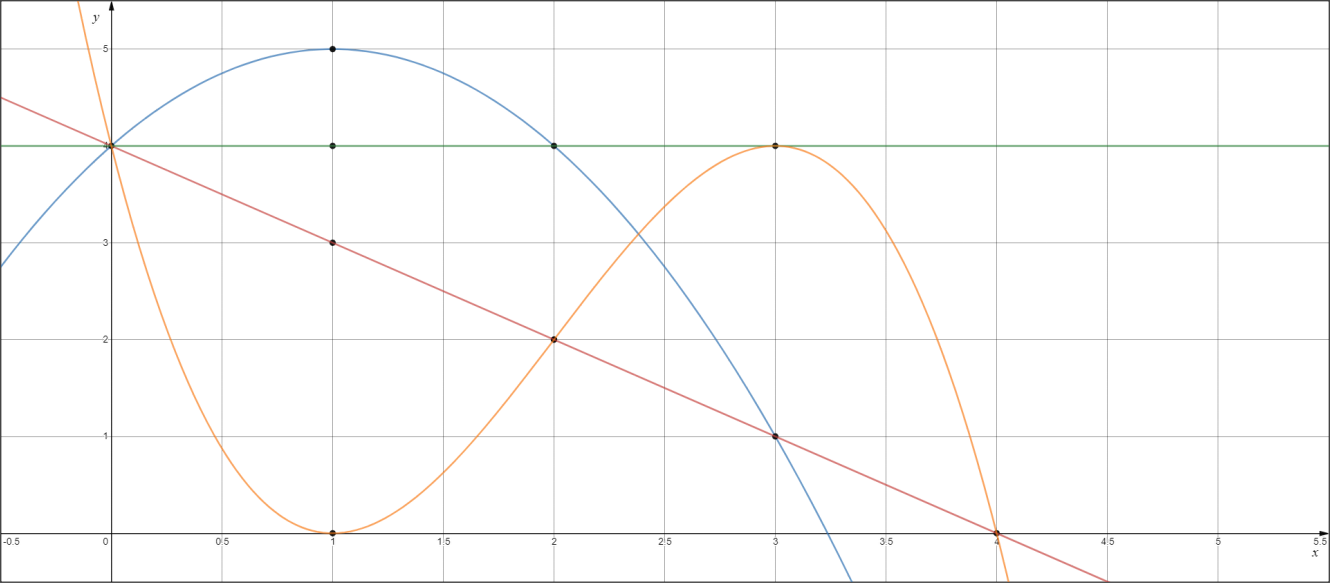
\includegraphics[width=\linewidth]{plots/secretsharing_big.png}
  \caption{Shares for different $t$ with secret $s=4$}
  \label{fig:secretsharing}
\end{figure}

To recombine the secret, the parties simply broadcast or send their shares to a central entity, if more than $t$ shares are known, it suffices to calculate the Lagrange polynomial $p(x)$ and $s=p(0)$. In the case of not having enough shares, the Lagrange polynomial containing the secret becomes impossible to calculate since every polynomial is equally likely, thus revealing absolutely nothing about the secret.\\

Note that all arithmetic in this section can be done over some finite field $\mathbb{F}_q$ to speed up the algorithms.

A Generalisation of this $(t,n)$-Shamir secret sharing scheme from thesis \cite{de2012design} as follows (Protocol 2.1 and Protocol 2.2):
\begin{enumerate}
  \item \textbf{Share Generation:} To share $s \in \mathbb{F}_q$, the dealer generates random $a_1, ..., a_t \in \mathbb{F}_q$ and puts $p(x) = s + a_1x + ... + a_tx_t$. Then the dealer computes $[s]_i = p(i)$.
  \item \textbf{Share Distribution:} For each $i \in {1, ..., n}$, the dealer sends $[s]_i$ to party $P_i$.
  \item \textbf{Secret Reconstruction:} Let $D \subset {1, ..., n}$ be a set of size $t + 1$. Each party $P_i$ for $i \in D$ sends his share $[s]_i$ to all parties. Then, each party reconstructs the secret via Lagrange interpolation.
\end{enumerate}

%TODO add protocols from https://pure.tue.nl/ws/files/3430368/735328.pdf

In figure \ref{fig:secretsharing} a visualisation of this scheme shows us that in order to get the secret value, $s=4$ in this case, we need to know atleast $t+1$ points for a given $t$. The trivial case where $t=0$ (green line) is simple to understand. The secret is simply the y-value of the given point. Of course this is a rather useless approach to secret sharing since you are giving away the cleartext secret. The full potential of secret sharing becomes true for cases where $t>0$. Two points are needed for a first order polynomial (red line), three points for a second order polynomial and so on.\\
It's important to make sure the parties are distributed and to try minimizing the incentive to collude. Distribution is needed to lower the risk of having a malicious party taking over control of the network, this can be done by splitting the parties up to many small stakeholders instead of a couple centralized stakeholders. We can only totally avoid collusion if the secret holder partakes to the MPC.

\subsection{Operations}
A neural network can be seen as an enormous function with millions of coefficients. Lucky for us the function can be broken up into 3 different operations: addition and multiplication in fully connected and convolution layers and a relational operator for max pooling and ReLU activation function. We will now show how to securely compute each of these basic operations.

\subsubsection{Arithmetic operators}
Since Shamir's secrete sharing scheme is a linear sharing scheme, each party $Pi$ can locally compute any linear combination of a public or secret value with their secret share $[s]_i$. This gives us following operations:
\begin{itemize}
  \item \textbf{Addition of secret and public value ($[c] \gets [a] + \beta$):} Each party $P_i$ locally adds the public value $\beta \in \mathbb{F}_q$ to it's share $[a]_i$, resulting in the new share $[c]_i = [a]_i + \beta$. Since all parties add the same $\beta$, this value is a constant.
  \item \textbf{Multiplication of secret and public value ($[c] \gets [a] \cdot \beta$):} Each party $P_i$ locally multiplies the public (constant) value $\beta \in \mathbb{F}_q$ with it's share $[a]_i$, resulting in the new share $[c]_i = [a]_i \cdot \beta$.
  \item \textbf{Addition of multiple secrets ($[c] \gets [a] \cdot [b]$):} Each party $P_i$ locally adds it's secret shares $[a]_i$ and $[b]_i$, resulting in the new share $[c]_i = [a]_i + [b]_i$.
\end{itemize}

The last operation is visually demonstrated in figure \ref{fig:addsecrets}. In this example secret $a=1$ (green) and secret $b=3$ (red). After each party $P_i$ locally computes the addition of $[a]_i$ and $[b]_i$ and stores it as a new share $[c]_i$. After broadcasting the new, computated share $[c]$. They can recombine the shares via Lagrange interpolation to get the polynomial of the combined shares $[c]$ and more importantly the output of the addition of the two secrets $a$ and $b$. This happens all with zero knowledge about $a$ or $b$. Since the computations are done locally no communication other than the inital share distribution is needed, the round complexity is 1.
%TODO verify round complexity

\begin{figure}
  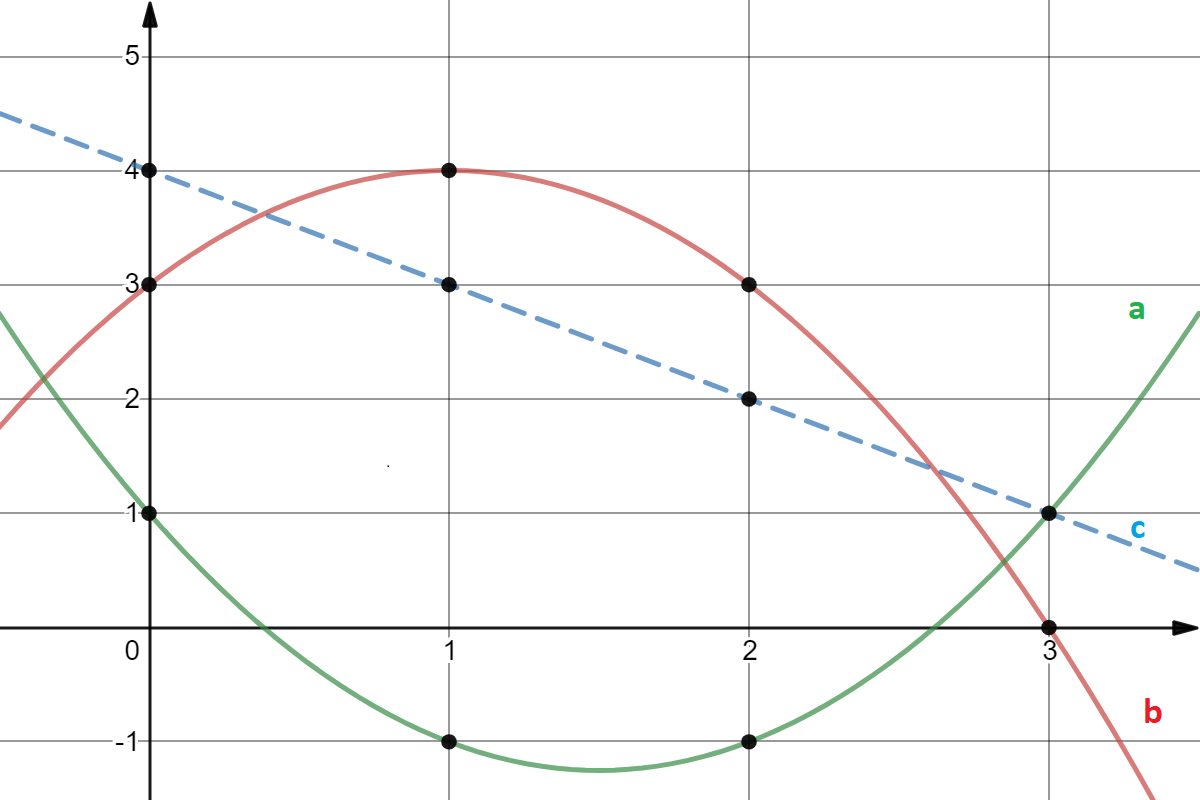
\includegraphics[width=\linewidth]{plots/addsecrets.png}
  \caption{Adding two secrets for $n=3$ parties}
  \label{fig:addsecrets}
\end{figure}

The inverse operations (subtraction and division) are possible too, and the protocol is the same.

\subsubsection{Relational operators}

\section{Related work}

\section{Conclusion}
